\documentclass[11pt]{article}

% some definitions for the title page
\newcommand{\reporttitle}{Self-supervised Learning}
\newcommand{\reportdescription}{This week's paper is~\cite{chen2020simple}}

% load some definitions and default packages
%---------------------------------------------------------------------------
%	PACKAGES AND OTHER DOCUMENT CONFIGURATIONS
%---------------------------------------------------------------------------

\usepackage[twoside]{fancyhdr}
\usepackage{csquotes}

\usepackage[a4paper,hmargin=2.0cm,vmargin=1.0cm,includeheadfoot]{geometry}
% \usepackage{natbib} % for bibliography
\usepackage{biblatex}
\usepackage{tabularx,longtable,multirow,subfigure,caption}%hangcaption
\usepackage{fancyhdr} % page layout
\usepackage{url} % URLs
\usepackage[english]{babel}
\usepackage{graphicx}
\usepackage{rotating}
\usepackage{dsfont}
\usepackage{epstopdf} % automatically replace .eps with .pdf in graphics
% \usepackage{backref} % needed for citations
\usepackage{array}
\usepackage{latexsym}
\usepackage[pdftex,hypertexnames=false,colorlinks]{hyperref} % provide links in pdf (had pagebackref)
\usepackage{booktabs}
\usepackage{wrapfig}
\usepackage{caption}  % Required for \captionof
\usepackage{float} % for H option in figures
\usepackage{amssymb}
\usepackage{amsmath}
\usepackage{amsthm}
\usepackage{mathtools} % for 'dcases*' env.
\usepackage[nottoc]{tocbibind}

%%% Default fonts
\renewcommand*{\rmdefault}{bch}
\renewcommand*{\ttdefault}{cmtt}

%%% Default settings (page layout)
\setlength{\parindent}{0em}  % indentation of paragraph
\setlength{\parskip}{.3em}
\setlength{\itemsep}{0.mm}

\setlength{\headheight}{14.5pt}
\pagestyle{fancy}

\fancyfoot[ER,OL]{\thepage}%Page no. in the left on odd pages and on right on even pages

\fancyfoot[OC,EC]{\sffamily }
\renewcommand{\headrulewidth}{0.1pt}
\renewcommand{\footrulewidth}{0.1pt}
\captionsetup{margin=10pt,font=small,labelfont=bf}

% LISTINGS ammendments
\usepackage{listings}
\usepackage{color}

\definecolor{mygreen}{rgb}{0,0.6,0}
\definecolor{mygray}{rgb}{0.5,0.5,0.5}
\definecolor{mymauve}{rgb}{0.58,0,0.82}

\lstset{ 
  postbreak=\mbox{\textcolor{red}{$\hookrightarrow$}\space},
  backgroundcolor=\color{white},   % choose the background color; you must add \usepackage{color} or \usepackage{xcolor}; should come as last argument
  basicstyle=\footnotesize,        % the size of the fonts that are used for the code
  breakatwhitespace=false,         % sets if automatic breaks should only happen at whitespace
  breaklines=true,                 % sets automatic line breaking
  captionpos=b,                    % sets the caption-position to bottom
  commentstyle=\color{mygreen},    % comment style
%   deletekeywords={...},            % if you want to delete keywords from the given language
%   escapeinside={\%*}{*)},          % if you want to add LaTeX within your code
  extendedchars=true,              % lets you use non-ASCII characters; for 8-bits encodings only, does not work with UTF-8
  firstnumber=1,                % start line enumeration with line 1000
  frame=single,	                   % adds a frame around the code
  keepspaces=true,                 % keeps spaces in text, useful for keeping indentation of code (possibly needs columns=flexible)
  columns=fullflexible,
  keywordstyle=\color{blue},       % keyword style
  language=python,                 % the language of the code
  % morekeywords={*,...},            % if you want to add more keywords to the set
  numbers=left,                    % where to put the line-numbers; possible values are (none, left, right)
  numbersep=5pt,                   % how far the line-numbers are from the code
  numberstyle=\tiny\color{mygray}, % the style that is used for the line-numbers
  rulecolor=\color{black},         % if not set, the frame-color may be changed on line-breaks within not-black text (e.g. comments (green here))
  showspaces=false,                % show spaces everywhere adding particular underscores; it overrides 'showstringspaces'
  showstringspaces=false,          % underline spaces within strings only
  showtabs=false,                  % show tabs within strings adding particular underscores
  stepnumber=1,                    % the step between two line-numbers. If it's 1, each line will be numbered
  stringstyle=\color{mymauve},     % string literal style
  tabsize=2,	                   % sets default tabsize to 2 spaces
  title=\lstname% show the filename of files included with \lstinputlisting; also try caption instead of title
}

% Here, you can define your own macros. Some examples are given below.

\newcommand{\R}[0]{\mathds{R}} % real numbers
\newcommand{\Z}[0]{\mathds{Z}} % integers
\newcommand{\N}[0]{\mathds{N}} % natural numbers
\newcommand{\C}[0]{\mathds{C}} % complex numbers
\renewcommand{\vec}[1]{{\boldsymbol{{#1}}}} % vector
\newcommand{\mat}[1]{{\boldsymbol{{#1}}}} % matrix


\bibliography{../bibliography}

\begin{document}

% Include the title page
\begin{titlepage}

    \newcommand{\HRule}{\rule{\linewidth}{0.5mm}} % Defines a new command for the horizontal lines, change thickness here
    
    \center % Center everything on the page
     
    %------------------------------------------------------------------------
    %	HEADING SECTIONS
    %------------------------------------------------------------------------
    
    \textsc{\Large Department of Computing}\\[0.5cm] 
    \textsc{\large Imperial College of Science, Technology and Medicine}\\[0.5cm] 
    
    %------------------------------------------------------------------------
    %	TITLE SECTION
    %------------------------------------------------------------------------
    
    \HRule \\[0.4cm]
    { \huge \bfseries \reporttitle}\\ % Title of your document
    \HRule \\[0.4cm]

    \textit{\reportdescription}
    
    \vspace{2em}

    %------------------------------------------------------------------------
    %	AUTHOR SECTION
    %------------------------------------------------------------------------
    
    \large \emph{Author: Anton Zhitomirskiy}

    \vspace{1em}

    \global\let\newpagegood\newpage
    \global\let\newpage\relax
    
\end{titlepage}

\global\let\newpage\newpagegood

\tableofcontents

\clearpage

\section{Motivation}

Supervised classifiers are very data hungry. This is a problem where labels are very expensive to acquire, but we have a lot of unlabelled images avialable (e.g. healthcare). The question is, could we learn to understand images without any labels?

\subsection{Standard supervised classification pipeline}

\begin{figure}[H]
    \centering
    \fbox{\includegraphics[page=4, trim=1cm 1.9cm 0.5cm 7.5cm, clip=true, width=.9\linewidth]{04 - Self-supervised learning.pdf}}
    \caption*{The question remains, `can we also learn useful image representation $h$ without labels?'}
\end{figure}

\subsection{Self-supervised learning classification pipeline}

\begin{figure}[H]
    \centering
    \fbox{\includegraphics[page=7, trim=1cm 3cm 0.5cm 6cm, clip=true, width=.9\linewidth]{04 - Self-supervised learning.pdf}}
    \caption*{We chop off the classificatio head becuase we don't ahve a label, so there is no classificaiton task, yet we still want to output a vector which summarises an image which still has all the important information to be used for classification as a downstream task. We require an objective for the network to strive for. Therefore we create proxys}
\end{figure}

\subsubsection{Proxy}

How can we create synthetic tasks that will get the network to learn useful representation?

\begin{itemize}
    \item \textbf{Contrastive-based learning}: teaching the network to recognise meaningful pairs of images (Section~\ref{sect:contrastive-based-learning}).
    \item \textbf{Generative-based learning}: teaching the network to reconstruct an image from a corrupted version (Section~\ref{sect:generative-based-learning})
    \item \textbf{Joint-Embedding Prediction}: a mix of both (Section~\ref{sect:joint-embedding-prediction}).
\end{itemize}

\section{Contrastive-based Learning | SIMCLR}\label{sect:contrastive-based-learning}

\subsection{Main Idea}

A meaningful representation should put similar images closer to each other.

\begin{figure}[H]
    \centering
    \fbox{\includegraphics[page=12, trim=0cm 0cm 10cm 9cm, clip=true, width=.9\linewidth]{04 - Self-supervised learning.pdf}}
    \caption*{However, without labels I don't know which images are dogs or cats so I cannot use this information as supervision signal!}
\end{figure}

\begin{figure}[H]
    \centering
    \fbox{\includegraphics[page=15, trim=0cm 0cm 10cm 7cm, clip=true, width=.9\linewidth]{04 - Self-supervised learning.pdf}}
    \caption*{The extra cat here is a blurred version of a cat already assigned to the circular space. Therefore, this perturbed versino of the same image should have a similar representation to the original image compared to all other images.}
\end{figure}

This is the main idea of contrastive-based learning: create multiple versions of the same image and theach the network to recognise the correct pair. The paper is at~\cite{chen2020simple}.

\subsection{Main Components}

\begin{figure}[H]
    \centering
    \fbox{\includegraphics[page=17, trim=3.4cm 3cm 5.4cm 6.4cm, clip=true, width=.9\linewidth]{04 - Self-supervised learning.pdf}}
    % \caption*{}
\end{figure}

\begin{enumerate}
    \item We are trying to pretrain the encoder $f(\cdot)$ that we are trying to train
    \item This encoder outputs a representation $h$ 
    \item Add small multi-layer perception to make the dimensions smaller. This is because in high diensional space, comparing similarities is harder, and not necessarily robust. This projector translates from vectors of size 2048 to 128 for example.
\end{enumerate}

\subsection{Walkthrough}

\begin{figure}[H]
    \centering
    \fbox{\includegraphics[page=19, trim=0cm 0cm 8.6cm 5.1cm, clip=true, width=.9\linewidth]{04 - Self-supervised learning.pdf}}
    \caption*{Start with two images $x_1 \wedge x_2$ and apply augmentations to them to produce (for example) two views. Then pass these images through the network. We want the embeddings of the two views of the cat to be close to each other, and at the same time have them far away from the dogs.}
\end{figure}

\begin{figure}[H]
    \centering
    \fbox{\includegraphics[page=19, trim=0cm 0cm 8.6cm 5.1cm, clip=true, width=.9\linewidth]{04 - Self-supervised learning.pdf}}
    \caption*{This is done for both of the views}
\end{figure}

\subsection{Augmentation Pipeline}

The augmentation you choose has very big consequences on what your model will actually learn. For example, an augmentation that removes colour will implicity teach the network that you should not care about the colour, only about the concept (shapes and textures).

We require the augmentation pipeline to:
\begin{itemize}
    \item Needs to reflect what information the model should diregard and what it should focus on
    \item Needs to be hard enough, otherwise trivial information is learnt.
\end{itemize}

\begin{figure}[H]
    \centering
    \fbox{\includegraphics[page=24, trim=11.8cm 1cm 0cm 6cm, clip=true, width=.9\linewidth]{04 - Self-supervised learning.pdf}}
    \caption*{These augmentation are very heavy, yet in the paper it is shown that this is what makes the model work}
\end{figure}

\subsection{Loss Function | NT-XNet loss}

\subsubsection{Similarity Measure}

The problem they try to solve is `how can we attract positive pairs while repelling negative pairs'. This is the \textbf{normalised temperature contrastive loss} algorithm.

\begin{equation}
    sim(\vec u, \vec v) = \frac{\vec u ^\top \vec v}{||\vec u|| \cdot ||\vec v||}
\end{equation}

This is essentially the cosine similarity which is the angle between the two vectors.

\subsubsection{Loss}

For each positive pair $(i,j)$ we have the following loss:

\begin{equation}
    \ell_{i,j} = - \log \frac{\exp(sim(\vec z_i, \vec z_j)/\tau)}{\sum^{SN}_{k=1} \vec 1_{[k\neq i]} \exp(sim(\vec z_i, \vec z_k)/\tau)} 
\end{equation}

\begin{enumerate}
    \item We want to minimise the loss, therefore we want to maximise the logarithm (since there is a leading $-$ in the loss function)
    \item Therefore, we need to maximise the numerator and minimise the denominator.
    \item \textbf{numerator}: We want to maximise the similarity (attract the embeddings we want together). I.e. maximise the nominator.
    \item \textbf{denominator}: Measure similairty between the first image and all other images in the batch. I.e. minimise the denominator.
    \item $\tau$ is the temperature, which controls how much to penalise hard negatives (negative pairs wrongly mapped close to each other). A low temperature penalises them more.
    \item here, $\textbf{1}_{[k\neq i]}$ is an indicator function evaluating to
    1 iff $k \neq i$ 
\end{enumerate}

The final loss is computed across all positive pairs, both $(i,j)$ and $(j,i)$, in amini-batch, by averaging all $l_{i,j}$.

\begin{figure}[H]
    \centering
    \fbox{\includegraphics[page=34, trim=1cm 0.5cm 4cm 5.2cm, clip=true, width=.9\linewidth]{04 - Self-supervised learning.pdf}}
    % \caption*{}
\end{figure}

\subsubsection{Triplet Loss}

\begin{equation}
    \mathcal L_{triplet}(\vec x, \vec x^+, \vec x^-)=\sum_{x\in \mathcal X}\max(0, ||f(x)-f(x^+)||^2_2 - ||f(x)-f(x^-)||^2_2+\epsilon)
\end{equation}

\begin{itemize}
    \item $x$ is one image
    \item $x^+$ is the corresponding positive
    \item $x^-$ is a randomly selected negative image
    \item $\epsilon$ is the marign parmeter controlling how far the negatives should be compared to the positive pairs (temperature $\tau$ plays this role in NT-Xent loss)
\end{itemize}

Here you want a similar thing: you wat the positive paris to be closer than the distance between the negatives (plus the margin). This qnautity is negative so the loss is zero. ``The positive pairs should be closer to eachother by at least $\epsilon$ margin compared to the distance to any negative pair''

\subsection{Evaluation of Self-supervised Learning}

\subsubsection{Finetuning}

\begin{figure}[H]
    \centering
    \fbox{\includegraphics[page=39, trim=2cm 0.5cm 3cm 5.2cm, clip=true, width=.9\linewidth]{04 - Self-supervised learning.pdf}}
    \caption*{}
\end{figure}

\subsubsection{Linear probing/evaluation}

\begin{figure}[H]
    \centering
    \fbox{\includegraphics[page=40, trim=2cm 0.5cm 3cm 5.2cm, clip=true, width=.9\linewidth]{04 - Self-supervised learning.pdf}}
    \caption*{``you can only base yourself on what you learned during the pre-training. So it cna be a good way to check what you're actually learning during the pretraining as opposed to if you do for fine tuning you might modify the encoder'' If you have few labels, then sometimes its better to keep the forzen encoder and just rtain the classificaiton label layer}
\end{figure}

\subsection{BatchSize}

To learn good representation, it is crucial to use very large batch sizes with SimCLR.

\begin{figure}[H]
    \centering
    \fbox{\includegraphics[page=41, trim=3cm 1cm 15cm 5.2cm, clip=true, width=.6\linewidth]{04 - Self-supervised learning.pdf}}
    \caption*{Linear evaluation | Key take-away; the more you pre-train the model, the better it gets. Also, bigger batch sizes learn a better representation of the image, the more images there are in your batch, the harder the task is.}
\end{figure}

\subsection{Follow-up work}

SimCLR requires very large batch size to provide good representation, this means very high computational requirements (expensive, difficult to train).

\subsubsection{Boostrap your won latent}

BYOL removes the need to use negative pairs in the loss function, instead one just optimises the similarity on the positive pairs $\rightarrow$ less need for bigger batch sizes. For that they need to introduce a new architecture to avoid learning trivial embeddings (otherwise all converge to the same point).

\begin{figure}[H]
    \centering
    \fbox{\includegraphics[page=44, trim=1cm 5cm 0.5cm 6cm, clip=true, width=.9\linewidth]{04 - Self-supervised learning.pdf}}
    \caption*{Where previously you would pass your two images into the same path, here we have them go itno two separate paths (because they might obtain the trivial solution). The student and teacher (as described above) the weights will not be the same so they won't return the same representation}
\end{figure}

\begin{figure}[H]
    \centering
    \fbox{\includegraphics[page=45, trim=1cm 5cm 0.5cm 6cm, clip=true, width=.9\linewidth]{04 - Self-supervised learning.pdf}}
    \caption*{``To further avoid the risk of still learning the trivial solution where these two just end up converging to the same point, they add yet another MLP (prediction) and try to match the output of online and target. You're trying to say that the output of the student network after the prediciton should be the same as the output of the target network without the prediction''}
\end{figure}

\begin{figure}[H]
    \centering
    \fbox{\includegraphics[page=46, trim=4cm 2.5cm 2cm 6cm, clip=true, width=.9\linewidth]{04 - Self-supervised learning.pdf}}
    \caption*{}
\end{figure}

\subsubsection{DINO}

Very similar to training BYOl, but using visial transformers as encoders. ``Becuase they use vision transfoemers they have access to this attention layer and os they can visualise the attention amp of the network when they create the self-supervised encoding, and by visualising these attention maps they can generate self-supervised segmentation maps''.

\begin{figure}[H]
    \centering
    \fbox{\includegraphics[page=47, trim=0cm 1cm 0cm 10cm, clip=true, width=.9\linewidth]{04 - Self-supervised learning.pdf}}
    \caption*{}
\end{figure}

\subsection{Conclusion}

Contrastive learning is one pretext task that has proven very useful in self-supervised learning, but its not the only way. In particular, it has some drawbacks such as large batch sizes, design of the augmentation pipeline etc.

\section{Generative-based Learning}\label{sect:generative-based-learning}

\subsection{Main-Idea}

Another way to use the image as supervision signal is to teach the network to reconstruct the original image from a masked image. 

\begin{figure}[H]
    \centering
    \fbox{\includegraphics[page=54, trim=3cm 2.5cm 3cm 8cm, clip=true, width=.9\linewidth]{04 - Self-supervised learning.pdf}}
    \caption*{Instead of using pairs, constructing pairs to teach the network to learn semantics, they teach the network to reconstruct the original image from a masked image.}
\end{figure}

\subsubsection{Vision transformers (refresher)}

\begin{figure}[H]
    \centering
    \fbox{\includegraphics[page=55, trim=5cm 1.8cm 6cm 6.5cm, clip=true, width=.9\linewidth]{04 - Self-supervised learning.pdf}}
    \caption*{``They start with one image, they cut it in different non-overlapping patchesthen they pass it through some embedding and then they get it into a transformer encoder, which ahs some attention layers, and the attention layers update the representation of that patch using the information from the other patches, and progressively it gets updated and then it learns useful representaiton of each of these single patches.''}
\end{figure}

\subsection{Masked Auto-encoders are scalable vision learners}

\begin{figure}[H]
    \centering
    \fbox{\includegraphics[page=59, trim=7cm 1.5cm 8cm 7cm, clip=true, width=.6\linewidth]{04 - Self-supervised learning.pdf}}
    \caption*{They divide the image in multiple subpatches and randomly mask some of the patches. After taking the patches they have, they feed it through the encoder which is a vision transformer. The encoder gets a representation for each patch and then you fill in the blanks iwth some mask token you learn during the process. The decoder then predicts each patch.
    
    The encoder here is drawn bigger becuase most of the computation is done in the encoder, and the decoder is pretty small. The goal is to put most of the details in the encoder (after training the decoder is thrown away).}
\end{figure}

\begin{figure}[H]
    \centering
    \fbox{\includegraphics[page=61, trim=1.4cm 2.5cm 1.7cm 6cm, clip=true, width=.9\linewidth]{04 - Self-supervised learning.pdf}}
    \caption*{The reconstruction of the detail is pretty bad, but this is because the size of the decoder is smaller (and we throw away the decoder after training)}
\end{figure}

\subsubsection{Loss}

\begin{equation}
    MSE = \sum(\hat x_i - x_i)^2,\quad \text{where $i$ is the pixel index}
\end{equation}

\subsubsection{Scalability}

\begin{figure}[H]
    \centering
    \fbox{\includegraphics[page=62, trim=8cm 1.8cm 8cm 5.5cm, clip=true, width=.5\linewidth]{04 - Self-supervised learning.pdf}}
    \caption*{The best result they got was approximately 75\% mask ratio}
\end{figure}

\subsection{Conclusion}

MAE avoids some of the drawbacks of CL, however, training a full reconstruction model is qute expensive. Maybe its not necessarily to full ylearn a perfect decoder model since we throw it away after training?

\section{Joint-Embedding Prediction}\label{sect:joint-embedding-prediction}

\subsection{i-Jepa}

Idea is to combine strength of CL and MAE approaches.

\begin{figure}[H]
    \centering
    \fbox{\includegraphics[page=66, trim=10.5cm 5.5cm 8cm 2cm, clip=true, width=.8\linewidth]{04 - Self-supervised learning.pdf}}
    \caption*{Some patches are masked, and we pass on the available patches to the context encoder. At the same time, we sample a region of the blue window, and pass it thorugh the target embedding. Repeat this for several regions. The goal of this paradigm is that instead of predicitng the missing image region, we are going to predict the encoded representation because the goal of the encoders is to summarise information, so instead of wasting compute reconstructing ever single pixel in the image, we are going to reconstruct the important information which there should be if the network is trained summarised.}
\end{figure}


\begin{figure}[H]
    \centering
    \fbox{\includegraphics[page=68, trim=8.7cm 2cm 8.5cm 5.5cm, clip=true, width=.8\linewidth]{04 - Self-supervised learning.pdf}}
\end{figure}

\subsubsection{Loss}

The loss is simply the average $L_2$ distance between the predicted patch-level representations $\hat s_y(i)$ and the target patch-level representation $s_y(i)$ i.e., 

\begin{equation}
    \frac 1 M \sum^N_{i=1}D(\hat s_y(i), s_y(i))=\frac 1 M \sum^M_{i=1}\sum_{j\in B_i} ||\hat s_{y_j} - s_{y_j} ||^2_2.
\end{equation}

\section{Examples in Healthcare}

\begin{figure}[H]
    \centering
    \fbox{\includegraphics[page=74, trim=3cm 3.5cm .5cm 5.5cm, clip=true, width=.95\linewidth]{04 - Self-supervised learning.pdf}}
\end{figure}

\begin{enumerate}
    \item ``Start by pretraining it on ImageNet (better performance than from scratch)''
    \item ``then they run SIMCLR from these weights. The goal is to go from a very generic encoder that has no idea baout medical languages to specialise it to learn on these unlablled chest x-rays''
    \item ``then they will use this on downstream tasks''
\end{enumerate}

\begin{figure}[H]
    \centering
    \fbox{\includegraphics[page=75, trim=6cm 2cm 7cm 6.7cm, clip=true, width=.95\linewidth]{04 - Self-supervised learning.pdf}}
    \caption*{Half a million scans were trained which didn't have labels, and saw that pre-training improved performance than from scratch.}
\end{figure}

\printbibliography
\addcontentsline{toc}{section}{Bibliography}

\end{document}